\documentclass{article}
\usepackage{tikz}
\usetikzlibrary{positioning, arrows.meta}

\begin{document}

\begin{tikzpicture}

% Draw timeline
\draw[line width=1mm, -{Stealth[length=2mm]}] (0,0) -- (10,0);

% Draw time intervals
\foreach \x/\y/\label in {1/6/{1970s}, 6/11/{1980s}, 11/16/{1990s}, 16/21/{2000s}, 21/26/{2010s}, 26/31/{2020s}, 31/36/{2030s}, 36/41/{2040s}, 41/46/{2050s}, 46/51/{2060s}}
  \draw (\x,0.3) -- (\x,-0.3) node[below] {\label};

% Draw events
\draw[fill=blue] (1,0) circle (4mm) node[above=0.4cm, align=center, text=white] {Moon\\ Landing};
\draw[fill=green] (5,0) circle (4mm) node[above=0.4cm, align=center, text=white] {Fall of\\ Berlin Wall};
\draw[fill=red] (10,0) circle (4mm) node[above=0.4cm, align=center, text=white] {World Wide\\ Web};
\draw[fill=orange] (20,0) circle (4mm) node[above=0.4cm, align=center, text=white] {Smartphones};
\draw[fill=purple] (30,0) circle (4mm) node[above=0.4cm, align=center, text=white] {Artificial\\ Intelligence};
\draw[fill=cyan] (40,0) circle (4mm) node[above=0.4cm, align=center, text=white] {Mars\\ Colonization};

\end{tikzpicture}

\end{document}
